The chapter presents an overview of the design of CacheInf.

\subsection{Working Environment and Metrics}
We assume that the working scenario of CacheInf is a mobile robot performing robotic tasks in a real-world field which requires real-time visual model inference on the continuous image stream captured from the on-board camera, to achieve real-time response to various environment changes.
The robot itself is equipped with low-power-consumption gpu to perform visual model inference which is slow and consumes too much power; it has wireless network access to a remote powerful GPU server that provides opportunity of acceleration, but the connection suffers from limited and unstable wireless network bandwidth.

While the requirements of real-time inference does not necessarily imply the requirement of high inference frequency, we measure the real-time metric by the average end-to-end inference latency when the robot is seamlessly performing inference, which leads to high inference frequency; the power consumption is also measured by average power consumption to finish inference on each image in the same scenario.

\subsection{Architecture of CacheInf}
To reduce inference latency by reusing cached previous computation results to both reduce local computation time and transmission time of offloading, CacheInf basically consists of three blocks: a scheduler, a cache tracker and an executor (TODO fix the names).

\begin{figure*}[!htb]
    \centering
    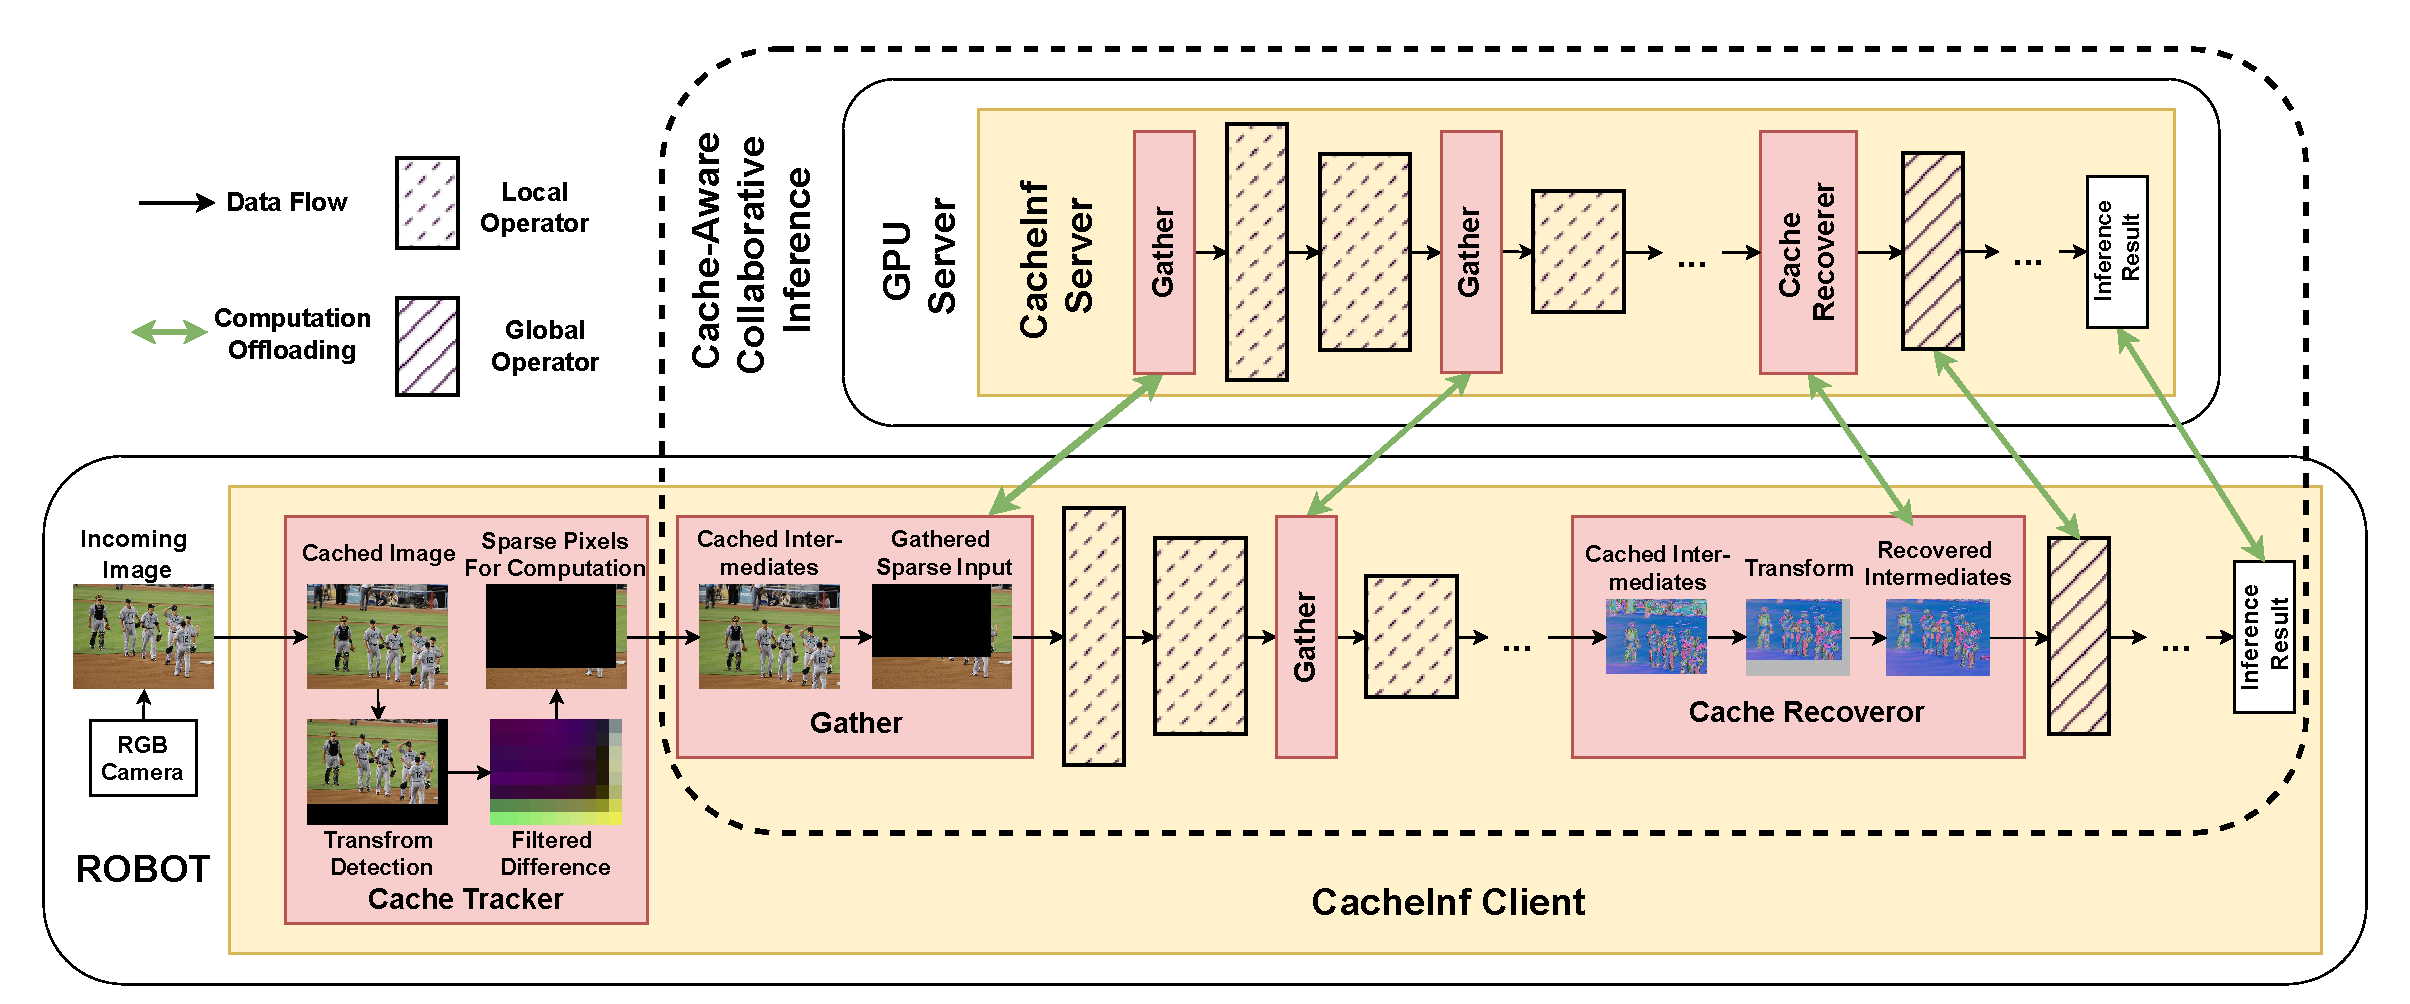
\includegraphics[width=\linewidth]{fig/overview.pdf}
    \caption[track]{Architecture and working process of CacheInf. TODO...}
    \label{fig:overview}
\end{figure*}

\subsubsection{Scheduler (TODO fix the names)}
During the initialization stage of the robotic task and CacheInf, CacheInf is granted access to the visual model and an initial input image and we mainly greedily pre-compute a schedule of various situations at this stage, since scheduling at runtime affects the real-time performance of the robotic task.
We first profile the model at both the robot and the remote GPU server to gather information  including shapes of the computation intermediates, the execution time of each operator (e.g., convolution, linear, etc.) on various scale of the input (e.g., from one tenth of the image to full scale of the image), the local property of each operator (i.e., whether the operator performs local computation) and so on.

Based on the above information, CacheInf finds sets of continuous local operators and assign the operators with smallest output sizes to be the operators to cache their computation results to reduce memory consumption of cache.
Then we coarsely iterate through the possible wireless network bandwidth, distribution of cache between the robot and the server and the portion of reusable cache and greedily compute a plan of whether to compute on cache and the portion of local computation and offloaded computation at the server at the reduced transmission data volume reusing cache.
We use the greedy strategy because we assume that both the wireless network bandwidth and the portion of reusable cache is unpredictable in the real-world scenario.
Note that the precomputed schedule can be reused for a same visual model with the same settings. 

\subsubsection{Cache Tracker}
At runtime, the selected operators at the previous stage will cache their computation results and the cache tracker identifies the reusable portion of such cached computation results.
Given an input image, we extract and store its features using classic computation vision methods (we choose Flann algorithm in our implementation, which is state-of-the-art).
For a current next image, we also extract and store its features and match them with the previous features (e.g., using KNN algorithm) and compute a perspective transform between the two images, which transforms the previous image such that the transformed previous image partially overlaps the current image and the non-overlapping areas are also marked.
The features of the previous images is then discarded.
The same transform can also be applied to the cached computation results since they are computed by local operators that keep the local geometries of the input image, and thus the reusable cached computation results are identified.
Note that the computation involved in this process is light-weight compared with the visual model inference that typically involves hundreds of operators.

\subsubsection{Executor (TODO fix the names)}
The executor is responsible to actually select and execute an plan based on results of the above two processes at runtime.
First, we further estimate the actual possible speedup by reusing cache, because the areas without cache needed for computation are often sparse and fragmented.
We cluster the areas without cache into different nearest clusters and compute minimum bounding boxes for each of the clusters;
then we greedily break up and recombine these bounding boxes to form a minimum new rectangle as a temporary input for the local operators and estimate its execution time based on its shape and the profile results from the initialization stage and select a precomputed plan for this input shape.
If no evident speedup, we will ignore the cache and use the whole input.

With a selected plan where cache is enabled, the executor reuses the temporary input of reorganized areas without cache described above and feed it into the inference pipeline; it also handles the portion of local computation and the portion of offloaded computation to the remote GPU server.
When appropriate, the executor breaks up the computation results of the temporary input and combines them with the transformed cache to recover geometries of the input image to get the correct result.
With a selected plan where cache is disabled, the actions with cache involved are excluded, but note that in any cases, the cache at the remote GPU server is always reused to reduce transmission data volume.









